\documentclass[conference]{IEEEtran}
\IEEEoverridecommandlockouts
% The preceding line is only needed to identify funding in the first footnote. If that is unneeded, please comment it out.
\usepackage{cite}
\usepackage{amsmath,amssymb,amsfonts}
\usepackage{algorithmic}
\usepackage{graphicx}
\usepackage{textcomp}
%idioma español
\usepackage[spanish]{babel} %ESPAÑOL
\usepackage[utf8]{inputenc}
\usepackage{float}
\usepackage{color}

%%
\def\BibTeX{{\rm B\kern-.05em{\sc i\kern-.025em b}\kern-.08em
    T\kern-.1667em\lower.7ex\hbox{E}\kern-.125emX}}
\begin{document}

\title{Bases de Datos Orientada a Grafos\\
Neo4j\\
%{\footnotesize \textsuperscript{*}Note: Sub-titles are not captured in Xplore and should not be used}
%\thanks{Identify applicable funding agency here. If none, delete this.}
}

\author{\IEEEauthorblockN{1\textsuperscript{ra} Laura Camila Scarpetta Rodríguez}
\IEEEauthorblockA{\textit{Universidad Distrital Francisco José de Caldas} \\
\textit{Maestría en Ciencias de la Información y la Comunicación}\\
Bogotá D.C., Colombia \\
lcscarpettar@correo.udistrital.edu.co}
\and
\IEEEauthorblockN{2\textsuperscript{do} José Manuel Vargas Montero}
\IEEEauthorblockA{\textit{Universidad Distrital Francisco José de Caldas} \\
\textit{Maestría en Ciencias de la Información y la Comunicación}\\
Bogotá D.C., Colombia \\
jomvargasm@correo.udistrital.edu.co}
}

\maketitle

\begin{abstract}
En este documento se verá una introducción al concepto de bases de datos orientada a grafos. Luego se hablará sobre la base de datos Neo4j. Se explicará su proceso de instalación para diferentes sistemas operativos y sus configuraciones iniciales. Posterior a ello se mostrará un manejo básico con este gestor de base de datos.
\end{abstract}

\begin{IEEEkeywords}
Neo4j, BDOG, base de datos, relaciones, consultas
\end{IEEEkeywords}

\section{Introducción}

Las bases de datos orientadas a grafos ofrecen una gran oportunidad en la actualidad en la que tenemos una creciente cantidad de información. \\
Este modelo ofrece tantas ventajas, como lo pueden resumir las famosas cuatro V: volumen, velocidad, veracidad y variedad. \\
Este modelo de bases de datos se puede implementar por medio de diferentes gestores de bases de datos.  Uno de los que toma gran importancia es Neo4j, por ser este de los pocos de OpenSource existentes.\\
Neo4j inició en el año 2007. Opera sobre Java. Es un sistema multiplataforma, desarrollado por la empresa Neo Technology. \\
Como ejemplo de su gran importancia y rápido crecimiento se debe decir que Neo4j tiene como clientes a las empresas Hewlett-Packard, eBay y Cisco.\\
En la Figura \ref{fig1} se observa el logo del software Neo4j.

\begin{figure}[H]
\begin{center}

\includegraphics[width= 0.45 \textwidth]{neo4j_logo.png}
\end{center}
\caption{Logo de Neo4j.}
\label{fig1}
\end{figure}


\section{Bases de datos orientadas a grafos}

Las bases de datos orientadas a grafos (DBOG) cambian el concepto completamente de las bases de datos relacionales (SQL) y hasta de las bases de datos no relaciones (NoSQL). La información, los objetos, de la base de datos se representan por nodos. Las relaciones entre los objetos se relacionan en los grafos con las aristas. Un ejemplo de un diagrama de grafos para una base de datos se muestra en la Figura \ref{fig2}.

\begin{figure}[H]
\begin{center}
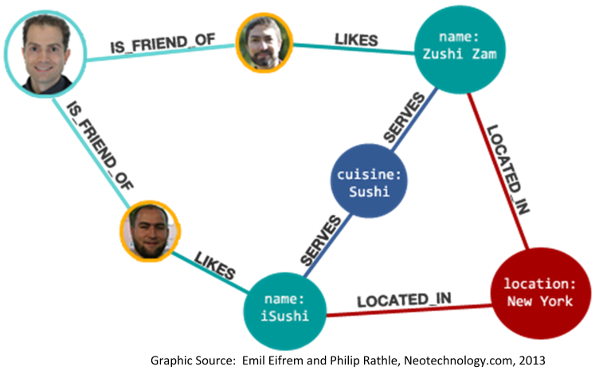
\includegraphics[width= 0.45 \textwidth]{graphDB.png}
\end{center}
\caption{Ejemplo de una DBOG.}
\label{fig2}
\end{figure}

Como se observa, el diagrama es bastante intuitivo de lo que nosotros entendemos por una relación. \\
Neo4j usa grafos de propiedad. Son grafos con peso, con etiquetas y donde podemos asignar propiedades tanto a nodos como relaciones (por
ejemplo, cuestiones como nombre, edad, país de residencia,nacimiento). 


\section{Instalación}
El proceso de instalación del programa Neo4j es diferente para cada sistema operativo. En el presente documento se explicará el proceso para la instalación en Windows y en una distribución de Linux (Ubuntu).\\
Se recomienda visitar la página de Neo4j para mayor información: 
\begin{itemize}
\item Requerimientos: https://neo4j.com/docs/operations-manual/current/installation/requirements/ 
\item Instalación para distribuciones Linux de Debian (Ubuntu):  https://neo4j.com/docs/operations-manual/current/installation/linux/debian/
\item Instalación para sistemas Window: https://neo4j.com/docs/operations-manual/current/installation/windows/
\end{itemize}

\subsection{Instalación en Windows}\label{AA}
Para instalar Neo4j en un computador (o servidor) con Windows se debe descargar el instalador de la página: https://neo4j.com/download/ \\
Una vez se haya descargado, se debe dar doble clic para ejecutarlo y se deben seguir las instrucciones. \\
Después de aceptar el acuerdo de licencia se mostrará la siguiente ventana, como se observa en la Figura \ref{fig3}.

\begin{figure}[H]
\begin{center}
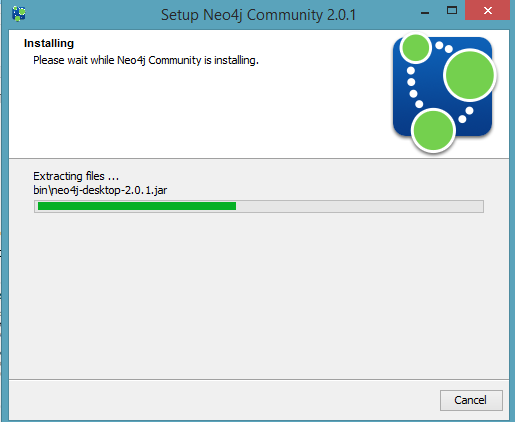
\includegraphics[width= 0.45 \textwidth]{neo4j_install02.png}
\end{center}
\caption{Instalación de Neo4j en Windows.}
\label{fig3}
\end{figure}

Una vez termine el proceso de instalación, se debe ejecutar Neo4j. Se abrirá la ventana que se muestra en la Figura \ref{fig4}.

\begin{figure}[H]
\begin{center}
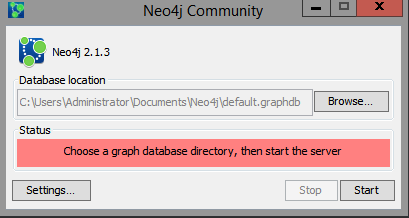
\includegraphics[width= 0.45 \textwidth]{neo4j_install06.png}
\end{center}
\caption{Ejecución de Neo4j en Windows.}
\label{fig4}
\end{figure}

Si se desea realizar configuraciones como
la cantidad de memoria RAM asignad a los nodos y las aristas, la configuración del acceso desde el explorador o desde un sitio remoto, el puerto de la conexión a la base de datos, habilitar auto indexación, entre otras opciones, se debe dar clic en Settings... Se desplegará una ventana como la que se muestra en la Figura \ref{fig5}.

\begin{figure}[H]
\begin{center}
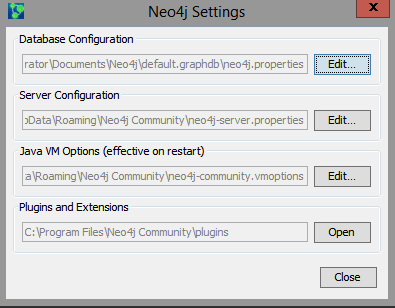
\includegraphics[width= 0.45 \textwidth]{neo4j_install07.png}
\end{center}
\caption{Configuraciones de Neo4j en Windows.}
\label{fig5}
\end{figure}

Finalmente, hechas las configuraciones deseadas, se debe dar clic en Start para hacer que el servidor arranque. La ventana de Neo4j debe quedar como en la Figura \ref{fig6}.

\begin{figure}[H]
\begin{center}
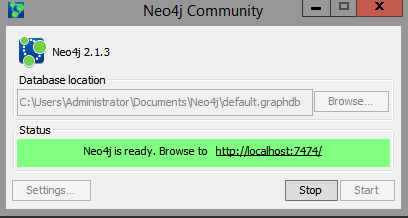
\includegraphics[width= 0.45 \textwidth]{neo4j_install09.png}
\end{center}
\caption{Arranque de Neo4j en Windows.}
\label{fig6}
\end{figure}

\subsection{Instalación en Linux (Debian/Ubuntu)}

Para las distribuciones de Linux el proceso es diferente. Es recomendable ir a la página https://neo4j.com/docs/operations-manual/current/installation/linux/debian/ para mayor información. \\
Para instalarlo se debe cumplir con el requisito de tener instalado Java 8 runtime. Para ello se debe ejecutar las siguientes sentencias, para tener acceso al repositorio e Java 8, como se muestran en las Figuras \ref{fig7} y \ref{fig8} 


\begin{figure}[H]
\begin{center}
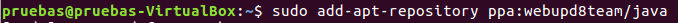
\includegraphics[width= 0.45 \textwidth]{java_repo.png}
\end{center}
\caption{Agregar repositorio de Java Runtime.}
\label{fig7}
\end{figure}

\begin{figure}[H]
\begin{center}
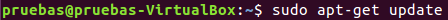
\includegraphics[width= 0.45 \textwidth]{sudo_update.png}
\end{center}
\caption{Actualizar repositorios de Linux.}
\label{fig8}
\end{figure}

Se usa la siguiente sentencia para poder instalar como tal el runtime de Java, como se observa en la Figura \ref{fig9}

\begin{figure}[H]
\begin{center}
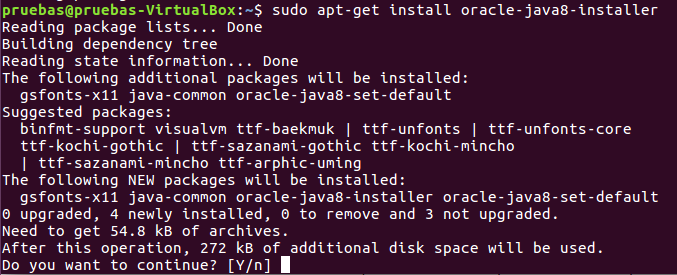
\includegraphics[width= 0.45 \textwidth]{install_java.png}
\end{center}
\caption{Instalación del Runtime de Java en Linux.}
\label{fig9}
\end{figure}

%sudo apt-get -t jessie-backports install ca-certificates-java

Una vez hecho esto, se debe agregar el repositorio de Neo4j. Para ello se ejecuta la siguiente sentencia desde la terminal, como se muestra en la Figura \ref{fig10}.

\begin{figure}[H]
\begin{center}
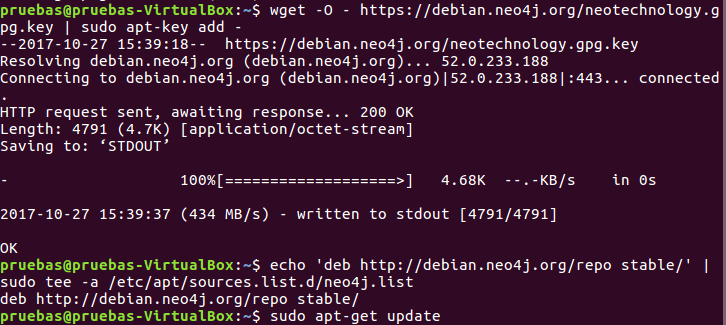
\includegraphics[width= 0.45 \textwidth]{neo4j_repo_f.png}
\end{center}
\caption{Repositorios de Neo4j en Linux.}
\label{fig10}
\end{figure}

Finalmente, se instala Neo4j, haciendo lo que se muestra en la Figura \ref{fig11}.

\begin{figure}[H]
\begin{center}
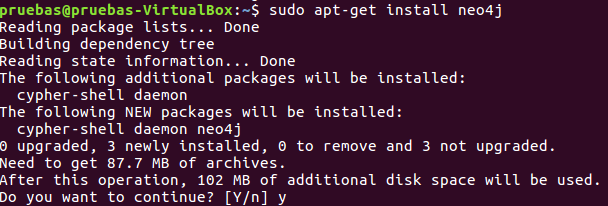
\includegraphics[width= 0.45 \textwidth]{install_neo4j.png}
\end{center}
\caption{Repositorios de Neo4j en Linux.}
\label{fig11}
\end{figure}

Para iniciar el servidor y arrancar en gestor de base de datos, se debe ejecutar el comando que se muestra en al Figura \ref{fig12}.

\begin{figure}[H]
\begin{center}
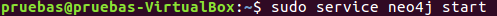
\includegraphics[width= 0.45 \textwidth]{start_service_neo.png}
\end{center}
\caption{Inicio del servidor de Neo4j en Linux.}
\label{fig12}
\end{figure}

\subsection{Prueba de la instalación}

Sin importar qué distribución  o qué sistema operativo se haya utilizado, se puede probar la correcta instalación utilizando el explorador Web. Se dirige a la dirección $localhost:7474/browser/$. 
\\
En esta dirección se tendrá todo el acceso y gestión de la base de datos: es un aplicativo corriendo sobre un explorador Web. Esto se muestra en la Figura \ref{fig13}.

\begin{figure}[H]
\begin{center}
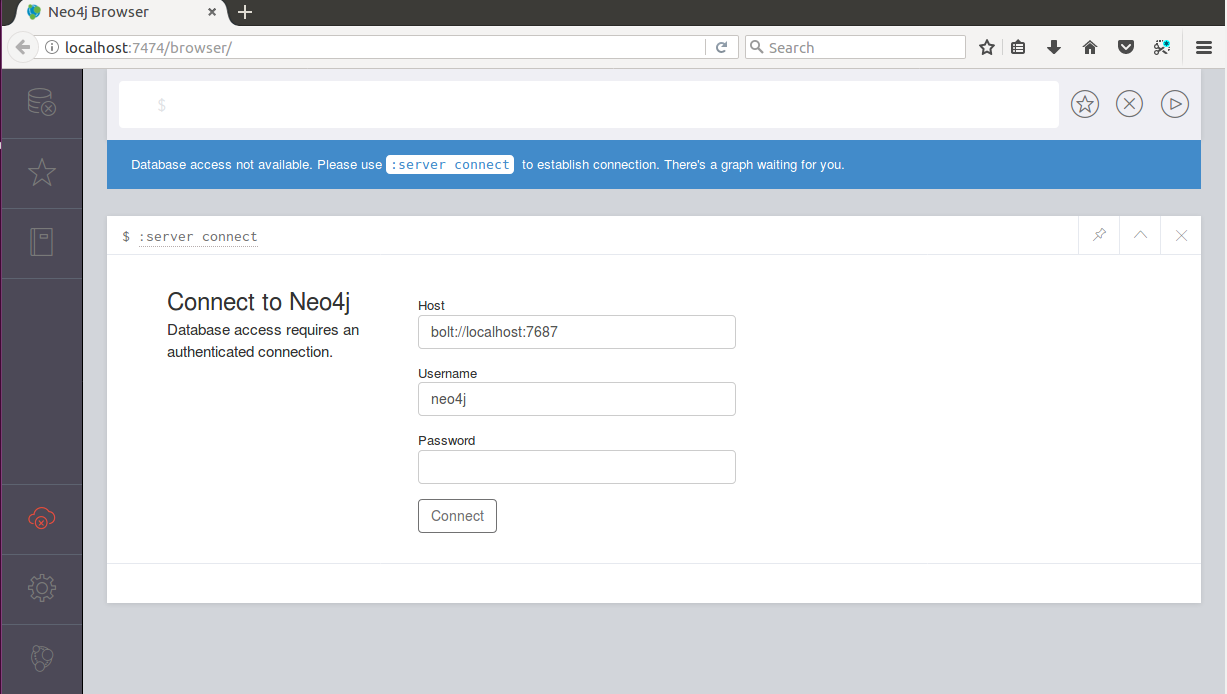
\includegraphics[width= 0.45 \textwidth]{web_browser1.png}
\end{center}
\caption{Neo4j corriendo desde el explorador Web.}
\label{fig13}
\end{figure}

La contraseña al iniciar Neo4j por primera vez por defecto es $neo4j$. Luego de ingresarla se pedirá se cambia la contraseña, como se muestra en la Figura \ref{fig14}.

\begin{figure}[H]
\begin{center}
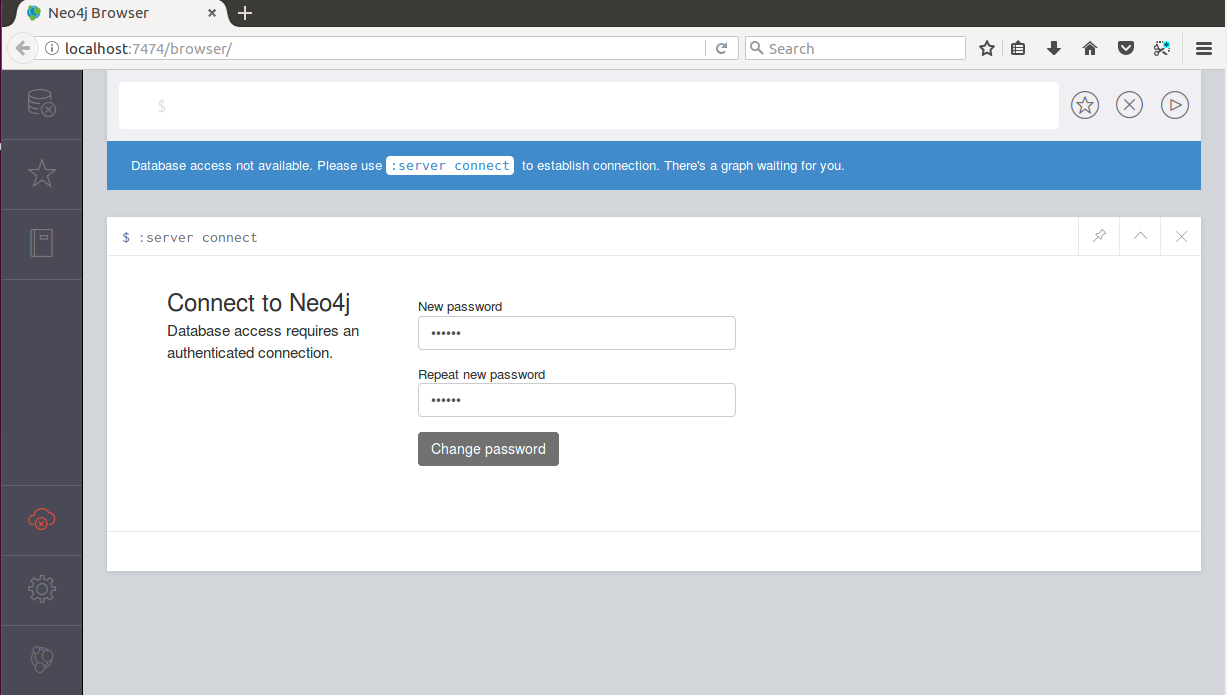
\includegraphics[width= 0.45 \textwidth]{web_change_p.png}
\end{center}
\caption{Cambio de contraseña en Neo4j por primera vez.}
\label{fig14}
\end{figure}

Una vez hecho esto, se estará en la página de inicio de Neo4j. Se verá la barra de ingreso de comandos (consultas), un espacio con las noticias y principales mensajes, un menú de accesos en el costado izquierdo y la conexión al servidor en sí. Todo esto se ilustra en la Figura \ref{fig15}.

\begin{figure}[H]
\begin{center}
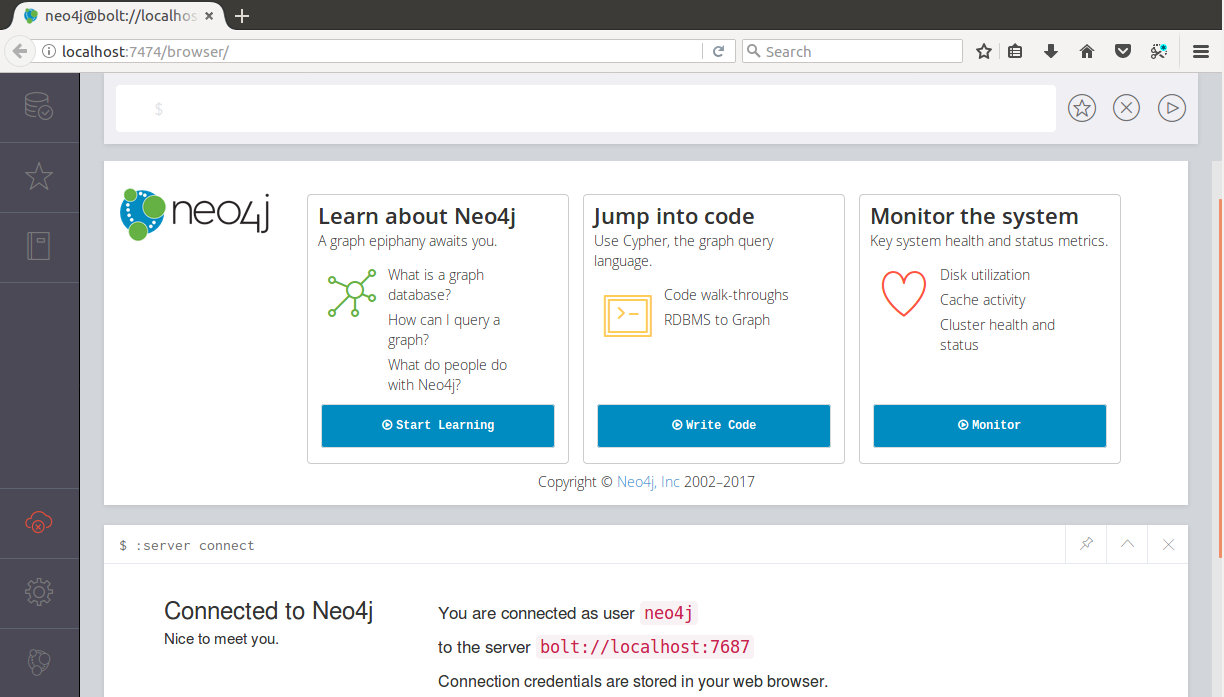
\includegraphics[width= 0.45 \textwidth]{inicio_neo4j.png}
\end{center}
\caption{Página de inicio de Neo4j.}
\label{fig15}
\end{figure}

\section{Creación de nodos.}

Una vez en el aplicativo de explorador se pueden crear nodos usando la sentencia \texttt{\textcolor{green}{CREATE} (\textcolor{blue}{n})}. Al ejecutar la sentencia se verá un mensaje que dice que se creó un nodo en un tiempo determinado. Si se desea observar el nodo, se debe crear de esta manera: \texttt{\textcolor{green}{CREATE} (\textcolor{blue}{n}) \textcolor{green}{RETURN} \textcolor{blue}{n}}. Esto se muestra en la Figura  \ref{fig16}.

\begin{figure}[H]
\begin{center}
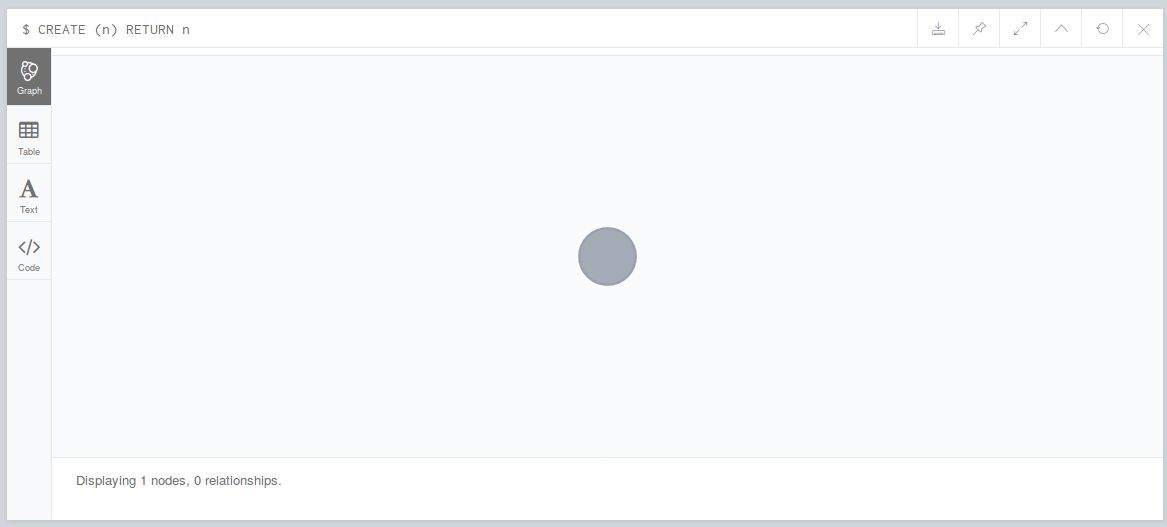
\includegraphics[width= 0.45 \textwidth]{create_node1.png}
\end{center}
\caption{Creación y visualización de un nodo.}
\label{fig16}
\end{figure}

Así mismo es posible crear varios nodos al tiempo y visualizarlos con el comando \texttt{\textcolor{green}{CREATE} (\textcolor{blue}{n}),(\textcolor{blue}{m}) \textcolor{green}{RETURN} \textcolor{blue}{n},\textcolor{blue}{m}}. 
\\
Un concepto importante en los nodos de Neo4j, son los label. Esta es una característica que define a qué grupo, clase o categoría pertenece el nodo. Por ejemplo, podemos crear nodos que pertenezcan y hagan referencia a personas. 
\\
Para agregar un label se hace de la siguiente manera: \texttt{\textcolor{green}{CREATE} (\textcolor{blue}{n}\textcolor{red}{:Persona}) \textcolor{green}{RETURN} \textcolor{blue}{n}}. Se debe aclarar aquí que la letra \texttt{n} es únicamente una referencia al nodo dentro de la sentencia específica. Bien se podría llamarlo o hacer referencia de otra manera y no cambiaría nada en el resultado. Por ejemplo \texttt{\textcolor{green}{CREATE} (\textcolor{blue}{yo}\textcolor{red}{:Persona}) \textcolor{green}{RETURN} \textcolor{blue}{yo}}. El resultado se muestra en la Figura \ref{fig17}.

\begin{figure}[H]
\begin{center}
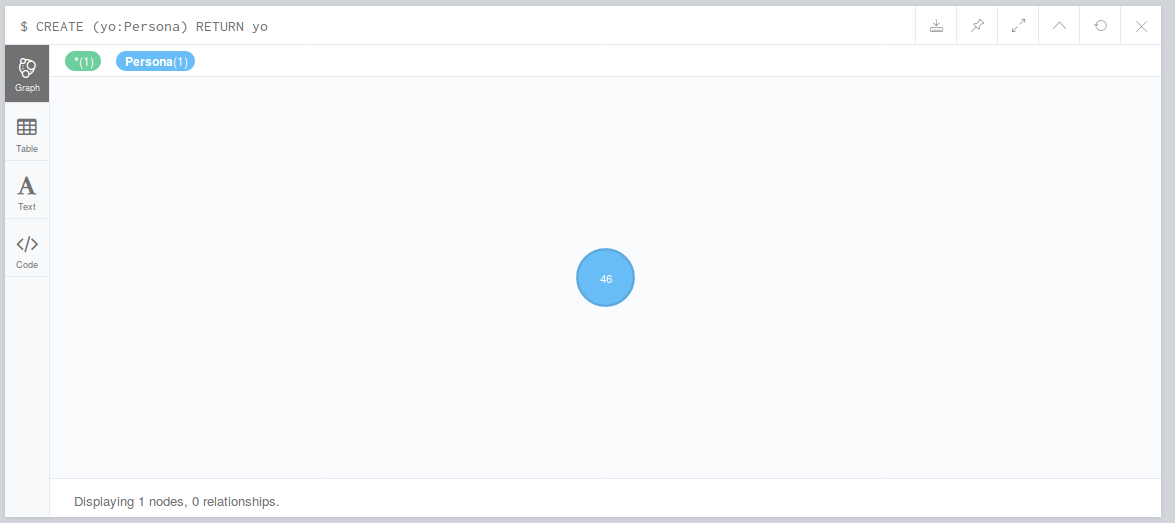
\includegraphics[width= 0.45 \textwidth]{crear_nodo_label1.png}
\end{center}
\caption{Nodo con label.}
\label{fig17}
\end{figure}

Dependiendo de la aplicación Neo4j permite tener más de un label para un nodo. Este sería el caso, por ejemplo, para nodos que pertenezcan a dos o más categorías. Un ejemplo sería una persona que tenga una nacionalidad. Esto se realiza agregando labels con : de manera consecutiva. Se puede usar la siguiente sentencia como ejemplo: \texttt{\textcolor{green}{CREATE} (\textcolor{blue}{persona}\textcolor{red}{:Persona:Colombia}) \textcolor{green}{RETURN} \textcolor{blue}{persona}}. Esto se observa en la Figura \ref{fig18}.

\begin{figure}[H]
\begin{center}
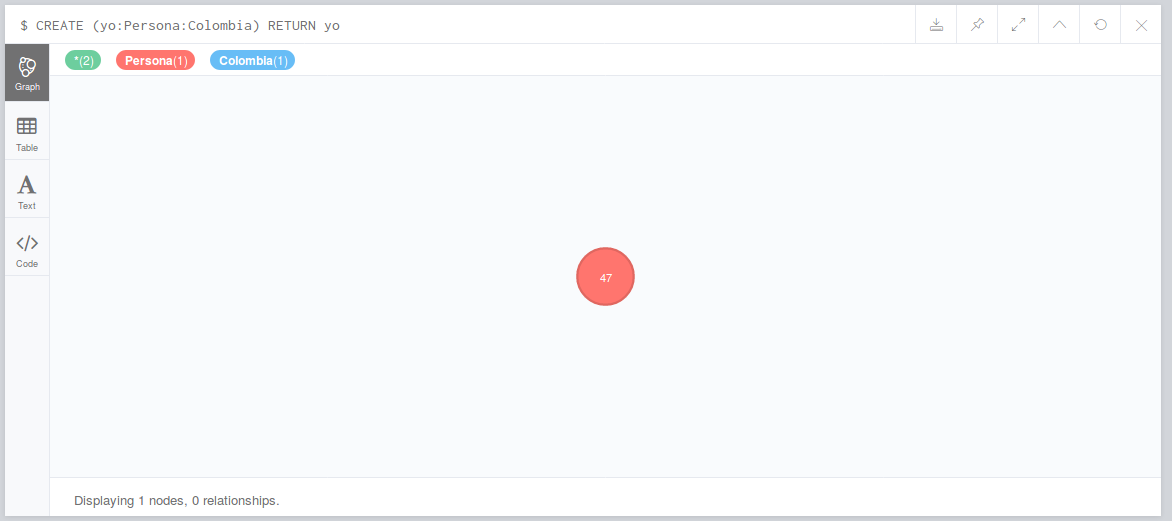
\includegraphics[width= 0.45 \textwidth]{crear_nodo_label2.png}
\end{center}
\caption{Nodo con dos label.}
\label{fig18}
\end{figure}



\subsection{Equations}
Number equations consecutively. To make your 
equations more compact, you may use the solidus (~/~), the exp function, or 
appropriate exponents. Italicize Roman symbols for quantities and variables, 
but not Greek symbols. Use a long dash rather than a hyphen for a minus 
sign. Punctuate equations with commas or periods when they are part of a 
sentence, as in:
\begin{equation}
a+b=\gamma\label{eq}
\end{equation}

Be sure that the 
symbols in your equation have been defined before or immediately following 
the equation. Use ``\eqref{eq}'', not ``Eq.~\eqref{eq}'' or ``equation \eqref{eq}'', except at 
the beginning of a sentence: ``Equation \eqref{eq} is . . .''

\subsection{\LaTeX-Specific Advice}

Please use ``soft'' (e.g., \verb|\eqref{Eq}|) cross references instead
of ``hard'' references (e.g., \verb|(1)|). That will make it possible
to combine sections, add equations, or change the order of figures or
citations without having to go through the file line by line.

Please don't use the \verb|{eqnarray}| equation environment. Use
\verb|{align}| or \verb|{IEEEeqnarray}| instead. The \verb|{eqnarray}|
environment leaves unsightly spaces around relation symbols.

Please note that the \verb|{subequations}| environment in {\LaTeX}
will increment the main equation counter even when there are no
equation numbers displayed. If you forget that, you might write an
article in which the equation numbers skip from (17) to (20), causing
the copy editors to wonder if you've discovered a new method of
counting.

{\BibTeX} does not work by magic. It doesn't get the bibliographic
data from thin air but from .bib files. If you use {\BibTeX} to produce a
bibliography you must send the .bib files. 

{\LaTeX} can't read your mind. If you assign the same label to a
subsubsection and a table, you might find that Table I has been cross
referenced as Table IV-B3. 

{\LaTeX} does not have precognitive abilities. If you put a
\verb|\label| command before the command that updates the counter it's
supposed to be using, the label will pick up the last counter to be
cross referenced instead. In particular, a \verb|\label| command
should not go before the caption of a figure or a table.

Do not use \verb|\nonumber| inside the \verb|{array}| environment. It
will not stop equation numbers inside \verb|{array}| (there won't be
any anyway) and it might stop a wanted equation number in the
surrounding equation.

\subsection{Some Common Mistakes}\label{SCM}
\begin{itemize}
\item The word ``data'' is plural, not singular.
\item The subscript for the permeability of vacuum $\mu_{0}$, and other common scientific constants, is zero with subscript formatting, not a lowercase letter ``o''.
\item In American English, commas, semicolons, periods, question and exclamation marks are located within quotation marks only when a complete thought or name is cited, such as a title or full quotation. When quotation marks are used, instead of a bold or italic typeface, to highlight a word or phrase, punctuation should appear outside of the quotation marks. A parenthetical phrase or statement at the end of a sentence is punctuated outside of the closing parenthesis (like this). (A parenthetical sentence is punctuated within the parentheses.)
\item A graph within a graph is an ``inset'', not an ``insert''. The word alternatively is preferred to the word ``alternately'' (unless you really mean something that alternates).
\item Do not use the word ``essentially'' to mean ``approximately'' or ``effectively''.
\item In your paper title, if the words ``that uses'' can accurately replace the word ``using'', capitalize the ``u''; if not, keep using lower-cased.
\item Be aware of the different meanings of the homophones ``affect'' and ``effect'', ``complement'' and ``compliment'', ``discreet'' and ``discrete'', ``principal'' and ``principle''.
\item Do not confuse ``imply'' and ``infer''.
\item The prefix ``non'' is not a word; it should be joined to the word it modifies, usually without a hyphen.
\item There is no period after the ``et'' in the Latin abbreviation ``et al.''.
\item The abbreviation ``i.e.'' means ``that is'', and the abbreviation ``e.g.'' means ``for example''.
\end{itemize}
An excellent style manual for science writers is \cite{b7}.

\subsection{Authors and Affiliations}
\textbf{The class file is designed for, but not limited to, six authors.} A 
minimum of one author is required for all conference articles. Author names 
should be listed starting from left to right and then moving down to the 
next line. This is the author sequence that will be used in future citations 
and by indexing services. Names should not be listed in columns nor group by 
affiliation. Please keep your affiliations as succinct as possible (for 
example, do not differentiate among departments of the same organization).

\subsection{Identify the Headings}
Headings, or heads, are organizational devices that guide the reader through 
your paper. There are two types: component heads and text heads.

Component heads identify the different components of your paper and are not 
topically subordinate to each other. Examples include Acknowledgments and 
References and, for these, the correct style to use is ``Heading 5''. Use 
``figure caption'' for your Figure captions, and ``table head'' for your 
table title. Run-in heads, such as ``Abstract'', will require you to apply a 
style (in this case, italic) in addition to the style provided by the drop 
down menu to differentiate the head from the text.

Text heads organize the topics on a relational, hierarchical basis. For 
example, the paper title is the primary text head because all subsequent 
material relates and elaborates on this one topic. If there are two or more 
sub-topics, the next level head (uppercase Roman numerals) should be used 
and, conversely, if there are not at least two sub-topics, then no subheads 
should be introduced.

\subsection{Figures and Tables}
\paragraph{Positioning Figures and Tables} Place figures and tables at the top and 
bottom of columns. Avoid placing them in the middle of columns. Large 
figures and tables may span across both columns. Figure captions should be 
below the figures; table heads should appear above the tables. Insert 
figures and tables after they are cited in the text. Use the abbreviation 
``Fig.~\ref{fig}'', even at the beginning of a sentence.

\begin{table}[htbp]
\caption{Table Type Styles}
\begin{center}
\begin{tabular}{|c|c|c|c|}
\hline
\textbf{Table}&\multicolumn{3}{|c|}{\textbf{Table Column Head}} \\
\cline{2-4} 
\textbf{Head} & \textbf{\textit{Table column subhead}}& \textbf{\textit{Subhead}}& \textbf{\textit{Subhead}} \\
\hline
copy& More table copy$^{\mathrm{a}}$& &  \\
\hline
\multicolumn{4}{l}{$^{\mathrm{a}}$Sample of a Table footnote.}
\end{tabular}
\label{tab1}
\end{center}
\end{table}

\begin{figure}[htbp]
\begin{center}
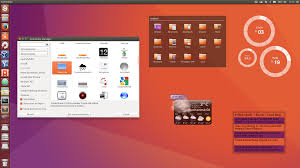
\includegraphics[width= 0.45 \textwidth]{fig2.jpeg}
\end{center}
\caption{Example of a figure caption.}
\label{fig}
\end{figure}

Figure Labels: Use 8 point Times New Roman for Figure labels. Use words 
rather than symbols or abbreviations when writing Figure axis labels to 
avoid confusing the reader. As an example, write the quantity 
``Magnetization'', or ``Magnetization, M'', not just ``M''. If including 
units in the label, present them within parentheses. Do not label axes only 
with units. In the example, write ``Magnetization (A/m)'' or ``Magnetization 
\{A[m(1)]\}'', not just ``A/m''. Do not label axes with a ratio of 
quantities and units. For example, write ``Temperature (K)'', not 
``Temperature/K''.

\section*{Acknowledgment}

The preferred spelling of the word ``acknowledgment'' in America is without 
an ``e'' after the ``g''. Avoid the stilted expression ``one of us (R. B. 
G.) thanks $\ldots$''. Instead, try ``R. B. G. thanks$\ldots$''. Put sponsor 
acknowledgments in the unnumbered footnote on the first page.

\section*{References}

Please number citations consecutively within brackets \cite{b1}. The 
sentence punctuation follows the bracket \cite{b2}. Refer simply to the reference 
number, as in \cite{b3}---do not use ``Ref. \cite{b3}'' or ``reference \cite{b3}'' except at 
the beginning of a sentence: ``Reference \cite{b3} was the first $\ldots$''

Number footnotes separately in superscripts. Place the actual footnote at 
the bottom of the column in which it was cited. Do not put footnotes in the 
abstract or reference list. Use letters for table footnotes.

Unless there are six authors or more give all authors' names; do not use 
``et al.''. Papers that have not been published, even if they have been 
submitted for publication, should be cited as ``unpublished'' \cite{b4}. Papers 
that have been accepted for publication should be cited as ``in press'' \cite{b5}. 
Capitalize only the first word in a paper title, except for proper nouns and 
element symbols.

For papers published in translation journals, please give the English 
citation first, followed by the original foreign-language citation \cite{b6}.


\begin{thebibliography}{00}
\bibitem{b1} G. Eason, B. Noble, and I. N. Sneddon, ``On certain integrals of Lipschitz-Hankel type involving products of Bessel functions,'' Phil. Trans. Roy. Soc. London, vol. A247, pp. 529--551, April 1955.
\bibitem{b2} J. Clerk Maxwell, A Treatise on Electricity and Magnetism, 3rd ed., vol. 2. Oxford: Clarendon, 1892, pp.68--73.
\bibitem{b3} I. S. Jacobs and C. P. Bean, ``Fine particles, thin films and exchange anisotropy,'' in Magnetism, vol. III, G. T. Rado and H. Suhl, Eds. New York: Academic, 1963, pp. 271--350.
\bibitem{b4} K. Elissa, ``Title of paper if known,'' unpublished.
\bibitem{b5} R. Nicole, ``Title of paper with only first word capitalized,'' J. Name Stand. Abbrev., in press.
\bibitem{b6} Y. Yorozu, M. Hirano, K. Oka, and Y. Tagawa, ``Electron spectroscopy studies on magneto-optical media and plastic substrate interface,'' IEEE Transl. J. Magn. Japan, vol. 2, pp. 740--741, August 1987 [Digests 9th Annual Conf. Magnetics Japan, p. 301, 1982].
\bibitem{b7} M. Young, The Technical Writer's Handbook. Mill Valley, CA: University Science, 1989.
\end{thebibliography}


\end{document}
